\documentclass[11pt]{article}
\usepackage{common}
\usepackage{hyperref}
\usepackage{graphicx}
\hypersetup{
    colorlinks=true,
    linkcolor=black,
    filecolor=magenta,      
    urlcolor=blue,
    citecolor=black
}
\setlength\parindent{0pt}
\setlength{\parskip}{1\baselineskip}
\title{On The Town: Social Planning as a Search Problem}
\author{Hakeem Angulu, Louie Ayre, and Amadou Camara}
\date{December 18, 2018}
\algtext*{EndWhile}% Remove "end while" text
\algtext*{EndIf}% Remove "end if" text
\algtext*{EndFor}% Remove "end for" text
\begin{document}
\maketitle{}

\tableofcontents

\newpage

\section{Introduction}

\textbf{On The Town (OTT)} is a web application designed to facilitate event planning between friends. Often, there are a variety of factors that complicate efforts to organize group outings. At what general location should the group meet to minimize travel without unfairly burdening some? What type of venue should be chosen to maximize utility? How much is everyone willing to spend? With \emph{OTT}, friends that are in the same city, but in different locations, can determine a venue  that is relatively equidistant from all people, and that also balances each user's preferences for type of activity, budget, and rating. 

Given a set of users spread out in various locations and information on venues and activities in a desired destinations, \emph{OTT} optimizes the process of meeting up with those that you care about. The problem of social planning here is well encoded as a search problem. \emph{OTT} uses a variety of search algorithms (including depth-first search, breadth-first search, uniform cost search, greedy search, and A* search) to output a list of 7 places that not only satisfy users' preferences, but are also diverse in their offerings. Thus, \emph{OTT} gives users a useful and varied set of options to execute.

The following is an example of the expected behavior: imagine $6$ friends scattered around New York City: uptown, downtown, midtown, etc. Based on the factors they decide, both through polls and preferences within their user profiles, \emph{OTT} minimizes the distance that each will have to travel in order to satisfy their desires, while also maximizing preference satisfaction and maintaining a diverse list of options. Given all of the users’ preferences, \emph{OTT} outputs $7$ locations. Then, the friends meet up and have a fun time!

\section{Background and Related Work}

Much of the background necessary for this project was gathered from the CS182 course material, including lectures and the textbook \cite{astar}. The developers were intrigued by the power of the search algorithms discussed and how different data structures could be utilized to adjust for the specifications of the problem at hand. The developers supplemented their understanding of these concepts with selections from \textit{A Dictionary of Computer Science} \cite{bfs_csdict}. When the complexity of designing an appropriate heuristic for this problem became apparent, \textit{A Formal Basis for the Heuristic Determination of Minimum Cost Paths} was useful for guidance and inspiration \cite{heuristic}.

\section{Problem Specification}

\textbf{Problem}: Given a set of preferences by a group of users, find a set of solutions that satisfies as many preferences as possible while maintaining diversity among the solutions in that set.

OTT encodes this problem as a search problem. As in other search problems, there are a few parameters, defined for this problem below:
\begin{itemize}
    \item a set of states: each state in this problem encodes a list of place for the users to visit
    \item a start state: an empty list
    \item a goal test: whether or not the length of the state is $7$, the desired number of solutions
    \item a successor function: a function that takes in the current path and returns a subset of all possible next places that are dissimilar from the current state. "Similarity" is defined by the similarity function which checks the attributes (price, rating, etc.) of a group of places and returns a list of places that have sufficiently different attributes. This allows OTT to produce a diverse set of solutions.
\end{itemize}

\section{Approach}

The \href{https://github.com/acamara1498/OTT}{production version of OTT} utilizes the A* search algorithm, which was chosen after the rigorous testing described below. The following are all the algorithms considered and studied for OTT:
\begin{itemize}
    \item Depth-First Search
    \item Breadth-First Search
    \item Greedy Search
    \item Uniform Cost Search
    \item A* Search
\end{itemize}

The following are the data structures that support the implementation of these algorithms and \emph{OTT}:
\begin{itemize}
    \item the $User$ class: Each user is initialized with their location and their preferences based on event, price, and ratings. This class has the following objects:
    \begin{itemize}
        \item $name$ (string): The user's name.
        \item $location$ (tuple): A tuple of latitude and longitude that encodes the user's location.
        \item $organizer$ (boolean): Whether or not the user is the organizer.
        \item $pricePref$ (int): The user's price preference as an integer between 0 and 4, inclusive.
        \item $ratingPref$ (float): The user's preference for a place's rating as a float between 1.0 and 5.0, inclusive.
        \item $eventPref$ (string): The user's preference for a type of event.
    \end{itemize}
    \item the $Party$ class: This holds the data about a given group of users including their center, a filtered list of places and more used to find the best events. This class has the following objects:
    \begin{itemize}
        \item $users$ (list): List of User objects.
        \item $center$ (tuple): Tuple of the center of all users' locations.
        \item $places$ (list): A list of potential places.
        \item $findCenter$ (method): The true center of geographical longitudes and latitudes.
        \item $addToParty$ (method): Add a user to the party.
        \item $searchLocation$ (method): Take the center location and search for all possible events within a given radius.
        \item $addPlaces$ (method): Iterate through the response data received from API calls and add the formatted places to the list of all the places.
        \item $updatePlaces$ (method): Iterate through all of the Google types and searches the location for each to give all possible locations in the area.
        \item $filterList$ (method): Check if events in the list of total places satisfy at least one user's preferences and add those events to a new list.
        \item $updateAll$ (method): Reset and repopulate the list of places.
        \item $getDist$ (method): Compare the distance that a user must travel to the location to the distance that a user must travel the geographical center.
        \item $sadnessFunction$ (method): Evaluate how each user in the party is affected by a specific event's type, price, rating, and distance, based on their preferences.
        \item $assignSadness$ (method): Assign a sadness list to each event.
    \end{itemize}
    \item the $Algorithm$ class: A container for different types of search algorithms.
    \begin{itemize}
        \item $type$ (string): A string denoting the type of algorithm.
        \item $cost\textunderscore fn$ (function): The cost function for the algorithm.
        \item $heuristic$ (function): The heuristic used for A* search.
        \item $dfsSearch$ (method): The DFS algorithm.
        \item $bfsSearch$ (method): The BFS algorithm.
        \item $greedySearch$ (method): The Greedy Search algorithm.
        \item $astarSearch$ (method): The A* Search algorithm.
        \item $ucsSearch$ (method): The UCS algorithm.
    \end{itemize}
    \item the $Stack$ class: A container with a last-in-first-out (LIFO) queuing policy.
    \item the $Queue$ class: A container with a first-in-first-out (FIFO) queuing policy.
    \item the $PriorityQueue$ class: Implements a priority queue data structure.
    \item the $PriorityQueueWithFunction$ class: Implements a priority queue with the same push/pop signature of the $Queue$ and the $Stack$ classes.
\end{itemize}

\newpage
The algorithms are discussed in detail below.

\bigskip

\textbf{Depth-First Search}

Depth-First Search (DFS) performs a search of a directed graph (or tree) by starting at the root node (or selecting some arbitrary node as the root node in the case of a graph) and exploring as far as possible along each branch before backtracking.\cite{dfs_csdict}

An initial starting vertex, $u = []$, is selected, its successors are generated and added to the frontier, and then it is "visited." The visit entails checking if the goal (a list of 7 solutions) has been met and logging that visit in a list. Then, each of the successors in the frontier is visited, and their successors are added to the frontier after each visit. In order to check all nodes at a certain branch, the frontier is traversed such that the last nodes added are the first ones removed (last-in first-out, FIFO), and thus encoded as a stack. The search terminates when the length of a node reaches $7$.

The time complexity of DFS is $O(b^m) = O(b^7)$ and the space complexity is $O(b*m) = O(b)$, where $b$ is the branching factor (the average number of successors per state) and $m=7$ is the max depth.

The algorithm is described with the Pythonic pseudocode below in \emph{Algorithm 1}, with the data structure, $dstruct$, instantiated as a $Stack$ object. 

\bigskip

\textbf{Breadth-First Search}

Breadth-First Search (BFS) performs a search of a directed graph (or tree) by starting at the root node and searching through the structure at level $k$ before proceeding to nodes at level $k+1$.\cite{bfs_csdict}

An initial starting vertex, $u = []$, is selected, its successors are generated and added to the frontier, and then it is "visited." The visit entails checking if the goal (a list of 7 solutions) has been met and logging that visit in a list. Then, each of the successors in the frontier is visited, and their successors are added to the frontier after each visit. In order to check all nodes at a certain depth, the frontier is traversed such that the first nodes added are the first ones removed (first-in first-out, FIFO), and thus encoded as a queue. The search terminates when the length of a node reaches $7$.

The time complexity of BFS is $O(b^m)$ and the space complexity is $O(b^m)=O(b^7)$, where $b$ is the branching factor (the average number of successors per state), and $m=7$ is the max depth.

The algorithm is described with the Pythonic pseudocode below in \emph{Algorithm 1}, with the data structure, $dstruct$, instantiated as a $Queue$ object. 

\medskip

\textbf{Greedy Search}

Greedy search performs a search of a directed graph (or tree) by starting at the root node and searching through the structure by visiting the nodes with the least value for the heuristic, $h(x)$, where $x$ is the successor node. For \emph{OTT}, the heuristic is described below in \emph{Algorithm 2}.

An initial starting vertex, $u = []$, is selected, its successors are generated and added to the frontier, and then it is "visited." The visit entails checking if the goal (a list of 7 solutions) has been met and logging that visit in a list. Then, each of the successors in the frontier is visited, and their successors are added to the frontier after each visit. In order to check the nodes that have the least value for the heuristic, the frontier is a priority queue where the priority is the value of the heuristic, and thus the node with the lowest value is removed first. The search terminates when the length of a node reaches $7$.

The time and space complexities of Greedy Search are determined by the heuristic, and thus cannot be reported with complete accuracy. Based on \emph{OTT}'s heuristic, the estimate of the upper bound of complexity for both time and space is $O(b^d) = O(b)$, where $b$ is the branching factor (the average number of successors per state), and $d$ is the depth of the solution $=7$.

The algorithm is described with the Pythonic pseudocode below in \emph{Algorithm 1}, with the data structure, $dstruct$, instantiated as a $PriorityQueue$ object. The push method of this object also takes an extra parameter, $h(x)$, the value of the heuristic at node $x$.

\medskip

\textbf{Uniform Cost Search}

Uniform cost search performs a search of a directed graph (or tree) by starting at the root node and searching through the structure by visiting the nodes with the least value for the cost function, $c(x)$, where $x$ is the successor node. For \emph{OTT}, the cost function is the sadness function described below, and in \emph{Algorithm 3}.

An initial starting vertex, $u = []$, is selected, its successors are generated and added to the frontier, and then it is "visited." The visit entails checking if the goal (a list of 7 solutions) has been met and logging that visit in a list. Then, each of the successors in the frontier is visited, and their successors are added to the frontier after each visit. In order to check the nodes that have the least value for the cost function, the frontier is a priority queue where the priority is the value of the cost function, and thus the node with the lowest cost is removed first. The search terminates when the length of a node reaches $7$.

The time complexity of UCS is $O(b^{c*/\epsilon})$ and the space complexity is $O(b^{c*/\epsilon})$, where $b$ is the branching factor (the average number of successors per state), $c*/\epsilon$ is the depth ($=7$), and $c*$ is the cost.

The algorithm is described with the Pythonic pseudocode below in \emph{Algorithm 1}, with the data structure, $dstruct$, instantiated as a $PriorityQueue$ object. The push method of this object also takes an extra parameter, $c(x)$, the value of the cost function at node $x$.

\medskip

\textbf{A* Search}

A* search performs a search of a directed graph (or tree) by starting at the root node and searching through the structure by visiting the nodes with the least value for the sum of the cost and heuristic functions, $h(x) + c(x)$, where $x$ is the successor node. For \emph{OTT}, the cost function is the sadness function described below and in \emph{Algorithm 3}, and the heuristic function is the function described below in \emph{Algorithm 2}.

An initial starting vertex, $u = []$, is selected, its successors are generated and added to the frontier, and then it is "visited." The visit entails checking if the goal (a list of 7 solutions) has been met and logging that visit in a list. Then, each of the successors in the frontier is visited, and their successors are added to the frontier after each visit. In order to check the nodes that have the least value for $f(x) = h(x) + c(x)$, the frontier is a priority queue where the priority is the value, $f(x)$, and thus the node with the lowest sum of cost and heuristic is removed first. The search terminates when the length of a node reaches $7$.

The time and space complexities of A* Search are determined by the heuristic (and the cost function), and thus cannot be reported with complete accuracy. Based on \emph{OTT}'s heuristic, the estimate of the upper bound of complexity for both time and space is $O(b^d)$. In the worst case of an unbounded search space, the number of nodes expanded is exponential in the depth of the solution (the shortest path) $d=7$: $O(b*d) = O(b)$, where $b$ is the branching factor (the average number of successors per state).\cite{astar}

The algorithm is described with the Pythonic pseudocode below in \emph{Algorithm 1}, with the data structure, $dstruct$, instantiated as a $PriorityQueue$ object. The push method of this object also takes an extra parameter, $f(x)$, the value of the sum of the cost and heuristic functions at node $x$. The cost and heuristic functions are described below, and in \emph{Algorithm 2} and \emph{Algorithm 3}.

\medskip

\textbf{Evaluation and Comparison}

The five algorithms above were run on random samples of parties to test their validity for this problem. At each step of these simulations, the average of the total sadness generated from the list of solutions served as a proxy for how well the algorithm did: the lower the average sadness, the closer the solutions were to satisfying all conditions, and the more satisfied the users. Another metric that was important was the time each algorithm takes to generate solutions, and that was also taken into account. Both are discussed below in the \textbf{Results} section.

\bigskip

\textbf{Sadness Function}

The cost function for the UCS and A* Search algorithms was the \emph{OTT} $sadnessFunction$ function. $sadnessFunction$ takes an $event$ and a $party$ object, and assigns a cost, or "sadness," for each user by taking a weighted combination of multiple measurements of its satisfaction of the user's preferences. The weights are:
\begin{itemize}
    \item the additional distance required for the user to travel with respect to the distance to center point of the party
    \item the difference in price between the user's budget and the venue's price rating
    \item the difference in rating between the user's preferred rating and the venue's rating
    \item whether or not the type of the venue is one of the user's preferred venue types
\end{itemize}

These weights were empirically determined by simulating $500$ random parties and averaging the $sadness$ attributed to each user for each event by the distance, price, rating, and type respectively. The resulting values were used to adjust the weights of each factor such that the inputs were comparable. 

The final sadness for a state, party configuration is the sum of each user's sadness, plus the sadness of the least satisfied user (the user with the highest sadness) to account for \emph{OTT}'s goal of minimizing total dissatisfaction while ensuring that  everyone in the party is at a reasonable threshold of satisfaction.

\bigskip 

\begin{algorithm}[!h]
  \begin{algorithmic}
    \Procedure{search}{$party$}
    \State{$visited \gets []$} \Comment{initialize variables to store the visited states and cost}
    \State{$cost \gets 0$}
    \State{$filteredList \gets party.filteredPlaces$} \Comment{the list of filtered places from party class}
    \State{$path \gets []$} \Comment{the starting path is an empty list}
    \State{$dstruct \gets Stack()$} \Comment{instantiate a frontier object}
    \State{$dstruct$.push(($path$, $filteredList$, $cost$))} \Comment{push the state to the frontier}
    \While{not $dstruct$.isEmpty}
        \State{$path$, $remaining$, $cost \gets$ $dstruct$.pop()} \Comment{get the next state from the frontier}
        \If{len($path$) $== 7$}
            \State{return $path$, $cost$} \Comment{check if at the goal}
        \Else
            \State{$event \gets path[-1]$} \Comment{if the list is not empty get the last element}
            \If{$event$ not in $visited$}
                \State{$visited$.append($event$)} \Comment{add the state to the visited list}
                \State{$nextList \gets$ $similarity$($event$, $remaining$)} \Comment{find the successors of the state}
                \For{$successor$ in $nextList$} \Comment{iterate through all successors}
                    \State{$sadness \gets successor["sadness"]$} \Comment{extract the sadness (cost) from the event}
                    \State{$nextCost \gets$ sum($sadness$) + max($sadness$)} \Comment{compute the cost}
                    \State{$dstruct$.push(($path + [successor]$, $nextList$, $cost + nextCost$))} \Comment{push the successor to the frontier}
                \Endfor
            \Else \Comment{if there are no events in the path}
                \For{$successor$ in $filteredList$}
                    \State{$sadness \gets successor["sadness"]$} \Comment{extract the sadness (cost proxy) from the event}
                    \State{$nextCost \gets$ sum($sadness$) + max($sadness$)} \Comment{compute the cost}
                    \State{$newList \gets$ copy.deepcopy($filteredList$)} \Comment{copy the list into a new structure}
                    \State{$newList$.remove($successor$)} \Comment{remove the successor from the list}
                    \State{$dstructk$.push(($path + [successor]$, $nextList$, $cost + nextCost$))} \Comment{push the successor to the frontier}
                \Endfor
            \Endif
        \Endif
    \Endwhile
    \EndProcedure{}
  \end{algorithmic}
  \caption{Search Algorithm}
\end{algorithm}

\begin{algorithm}[!h]
  \begin{algorithmic}
    \Procedure{heuristic}{$state$}
    \State{$progress \gets $ len($state[0]$)} \Comment{encode the progress to the goal as the length of the list of previous states}
    \If{$progress \neq 0$)} \Comment{Goal distance is the number of places left to be added multiplied by the average of the sadness value to the current point}
        \State{$goal\_distance = (7 - progress) * state[2] / progress$}
    \Else
        \State{$goal\_distance = 7$}
    \Endif
    \State{return: $goal\_distance$}
    \EndProcedure{}
  \end{algorithmic}
  \caption{Search Heuristic}
\end{algorithm}

\begin{algorithm}[!h]
  \begin{algorithmic}
    \Procedure{sadnessFunction}{$place$}
    \State $weight \gets \{"type": 0.319765608129, "price": 0.170200961101, "rating": 0.130747631926, "dist": 0.0156106747366\}$
    \Comment{weight the contributing factors to sadness}
    \State $sadness = [0] *$ len($self.users$) \Comment{initialize the sadness list}
    \For{$i$ in range(len($self.users$))}: \Comment{iterate through user list to calculate their sadness}
        \State{$dist$} \gets $self.$getDist($self.users[i]$, $place$)
        
        \If{$dist > 0$}: 
        \Comment{difference between distance to place and center}
            \State $sadness[i] += dist * weights["dist"] / normalizers["dist"]$
        \EndIf
        
        \State $rating$ \gets $self.users[i].ratingPref - place["rating"]$
        
        \If{$rating > 0$}: \Comment{difference between rating of place and rating preference}
            \State $sadness[i] += rating * weights["rating"] / normalizers["rating"]$
        \EndIf
        \State $price$ \gets float($place["price"] - self.users[i].pricePref$)
        
        \If{$price > 0$}: \Comment{difference between price of place and price preference}
            \State $sadness[i] += price * weights["price"] / normalizers["price"]$
        \EndIf
        \State $type \gets 0$
        \For{$event$ in $self.users[i].eventPref$}:
            \If{$event$ not in $place["types"]$}: \Comment{check if the type of the place is preferred}
                \State $type += 1$
            \EndIf
        \EndFor
        \If{$type == $ len($self.users[i].eventPref$)}:
            \State $type = 1$
        \Else
            \State $type = 0$
        \EndIf
    \EndFor
    \State return: $sadness$ \Comment{return a list of the sadness incurred by a place for each user in the party}
    \EndProcedure{}
  \end{algorithmic}
  \caption{Cost Function: Sadness}
\end{algorithm}

\newpage

\section{Experiments}

The algorithms take in a $Party$ object, which holds the data about a given group of users including their center, a filtered list of possible places, and preferences. In order to test the implementation and performance of the algorithms, data were generated to simulate many parties. $900$ parties were randomly created using a random party generator, described in \textit{Algorithm 4} below.

The following are the main aspects of a party that the algorithm creates:
\begin{itemize}
    \item location data for each user, randomly generated from a list of possible coordinates in New York City. New York City was used because it  was the impetus for this project, and it has a wide variety of available places
    \item activity type preference data for each user, randomly generated from a subset of the available activities Google encodes for the Google Places API
    \item rating preference data for each user, randomly generated from a list of $1$ to $4$
    \item price preference data for each user, randomly generated from a list of $1$ to $5$
    \item name, randomly created
\end{itemize}

These random processes allowed the developers to test a wide range of possibility automatically, streamlining assessment of both edge and general cases. Once these parties were created, each of the $5$ algorithms was run on them, and the following data for each were collected:
\begin{itemize}
    \item failure rate: the rate of failure of the algorithm, where failure is defined as taking more than $1$ minute to reach a solution, or returning an empty list (which was uncommon, but possible in \textit{BFS} and \textit{DFS} due to the design of the successor function
    \item evaluation time: the time it takes an algorithm to reach a solution
    \item the average sadness: the average sadness that a solution gave to the party to which it applies
\end{itemize}

All these data were saved in \texttt{simulated\_results.csv}, and the entire process can be replicated using the \texttt{evaluation.ipynb} Jupyter notebook. The analysis of the data lies in \texttt{analysis.ipynb}, and the major takeaways are reported below.

The evaluation and testing processes revealed a lot about the implementation, and a few changes had to be made along the way to handle edge cases the developers caught (for example, the case of returning no solutions, or the very long evaluation time of \textit{BFS}).

\begin{algorithm}[h!]
    \begin{algorithmic}
        \Procedure{randomParty}{num}
        \State{$coordList$} \gets[NY coords]
        \Comment{create list of various coordinates in NY city}
        \State{$typeList$} \gets[types]
        \Comment{create list of various type preferences}
        \State{$party$} $= Party()$
        \Comment{Initialize party}
        \State{$Coords$} \gets[]
        \Comment{Initialize empty list to hold party's coordinates}
        \For{$i$ in range($num$)}
            \State{$coord$} $=coordlist$[np.random.randint($0$,len($coordlist$))]
            \Comment{Get a user's unique coordinates}
            \While{$coord$ in $coords$}
              \State{$coords$} $=$ $coordlist$[np.random.randint($0$,len($coordlist$))]
            \EndWhile
            \State{$coords$.append($coord$)}
            \State{$username$} $=$ "User"+str($i$)
            \Comment{Assign a unique user name}
            \State{$rating$} $= 2 + 3*$np.random.random_sample()
            \Comment{Get rating preference, continuous [$2,5$]}
            \State{$price$} $=$ np.random.randint($1,5$)
            \Comment{Get price preference, discrete [$1,4$]}
            \State{$types$} $=$ np.random.choice($typelist,size =$ np.random.randint($1,4$),replace = False)
            
            \Comment{Get 1-3 type preferences}
            
            \State{$user$} $=$ c.User($username, coord[0], coord[1], price, rating, types$) 
            \Comment{Create user}
            \State{$party$.addToParty($user$)}
            \Comment{Add user to party}
        \EndFor
        \State{$party$.updateAll()}
        \Comment{Update Party}
        \State{return $party$}
    \end{algorithmic}
    \caption{Random Party Generator}
\end{algorithm}


\subsection{Results}

 For algorithm-comparison projects: a section reporting empirical comparison results preferably presented graphically.

The following outline the results of the tests described above. All numbers are given to three decimal places of precision.

\textbf{Failure Rate}

\textit{Table 1} describes the percentage of times the algorithms failed, where failure is defined as returning an empty list of solutions or taking more than $1$ minute to run. \textit{Figure 1} shows the graphical representation of this data. It is clear that \textit{BFS} is nearly unfeasible as an  algorithm for this project, failing nearly $90\%$ of the time. With more testing, the developers found that \textit{BFS} could sometimes take over $5$ hours to find a solution for a party of $6$. On the other hand, \textit{Greedy Search} performs the best, with a failure rate of only $14.889\%$.

\begin{table}[!h]
  \centering
  \begin{tabular}{l c}
    \toprule
    Algorithm & Failure Rate (\%) \\
    \midrule
    DFS & 32.000 \\
    BFS & 88.889 \\
    Greedy Search & 14.889 \\
    UCS & 39.667 \\
    A* Search & 15.889 \\
    \bottomrule
  \end{tabular}
  \caption{Failure Rate of Algorithms}
\end{table}

\begin{figure}[!h]
\centering
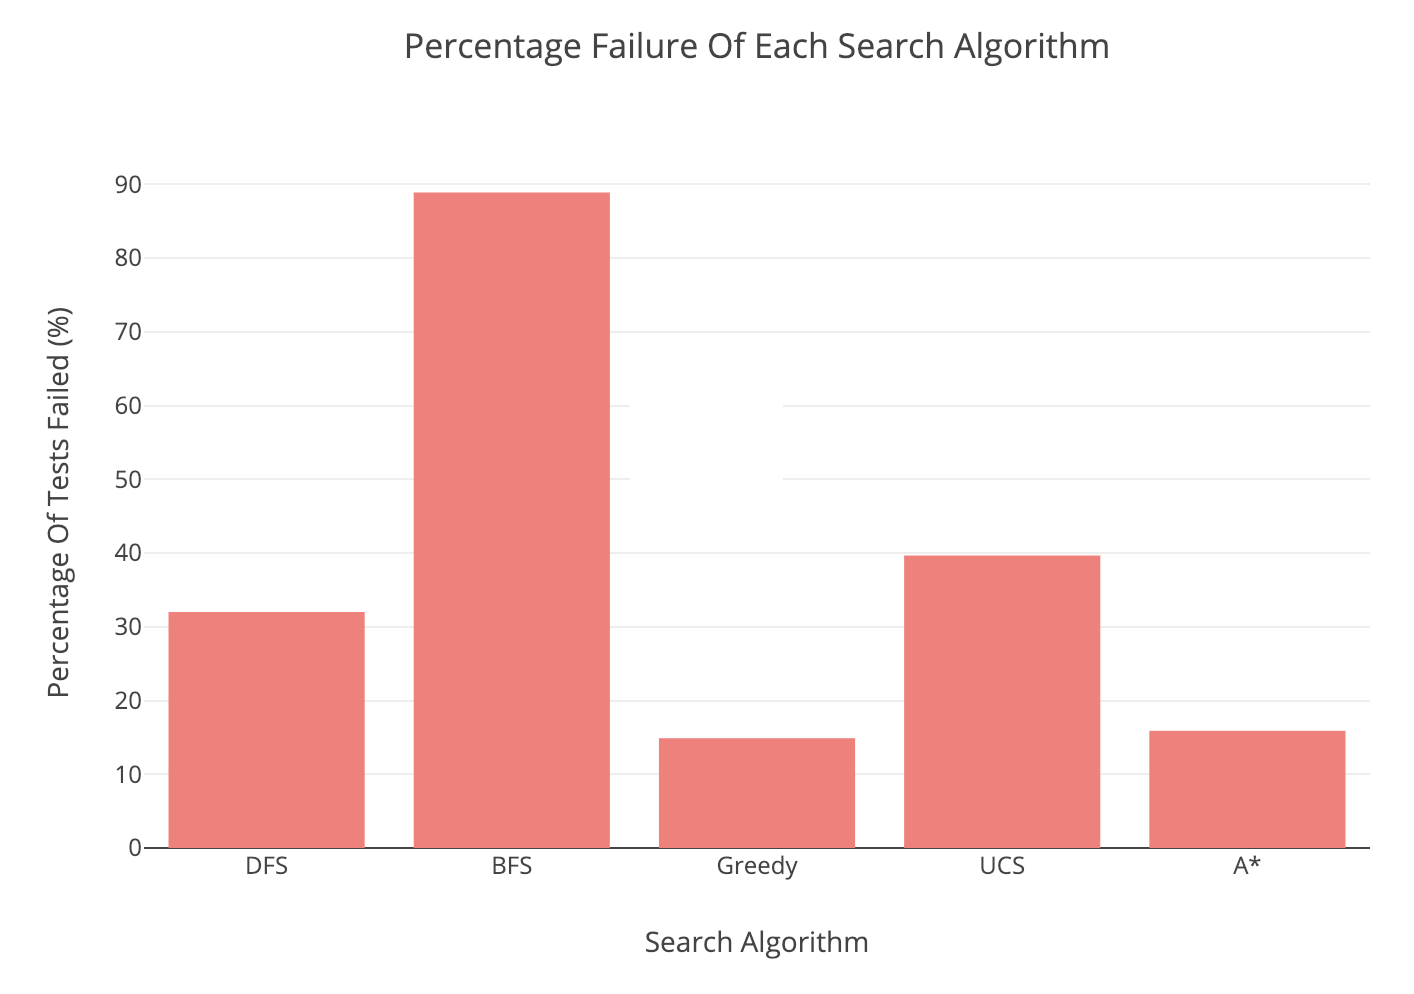
\includegraphics[width=\textwidth]{fail_bar.png}
\caption{Percentage Failure of Each Search Algorithm}
\end{figure}

\textbf{Evaluation Time}

\textit{Table 2} describes the average time in seconds that each algorithm took to find a solution when a solution was found. It is important to note that the times do not reflect the failure rate described above, and thus, the two should be interpreted together. \textit{Figure 2} shows the graphical representation of this data. To give further context to these point estimates, \textit{Figure 3} shows the distribution of the evaluation time as histograms. From these graphs, one can see that again, \textit{Greedy Search} performs remarkably well, and is the second fastest algorithm after \textit{DFS}, but with much more consistency towards good performance, as evidenced by the extreme right skew of the data. On the other hand, \textit{BFS} and \textit{UCS} are some of the worst performers.

\begin{table}[!h]
  \centering
  \begin{tabular}{l c}
    \toprule
    Algorithm & Average Evaluation Time (seconds) \\
    \midrule
    DFS & 0.289 \\
    BFS & 10.948 \\
    Greedy Search & 1.047 \\
    UCS & 15.108 \\
    A* Search & 3.0981 \\
    \bottomrule
  \end{tabular}
  \caption{Average Evaluation Time of Algorithms}
\end{table}

\begin{figure}[!h]
\centering
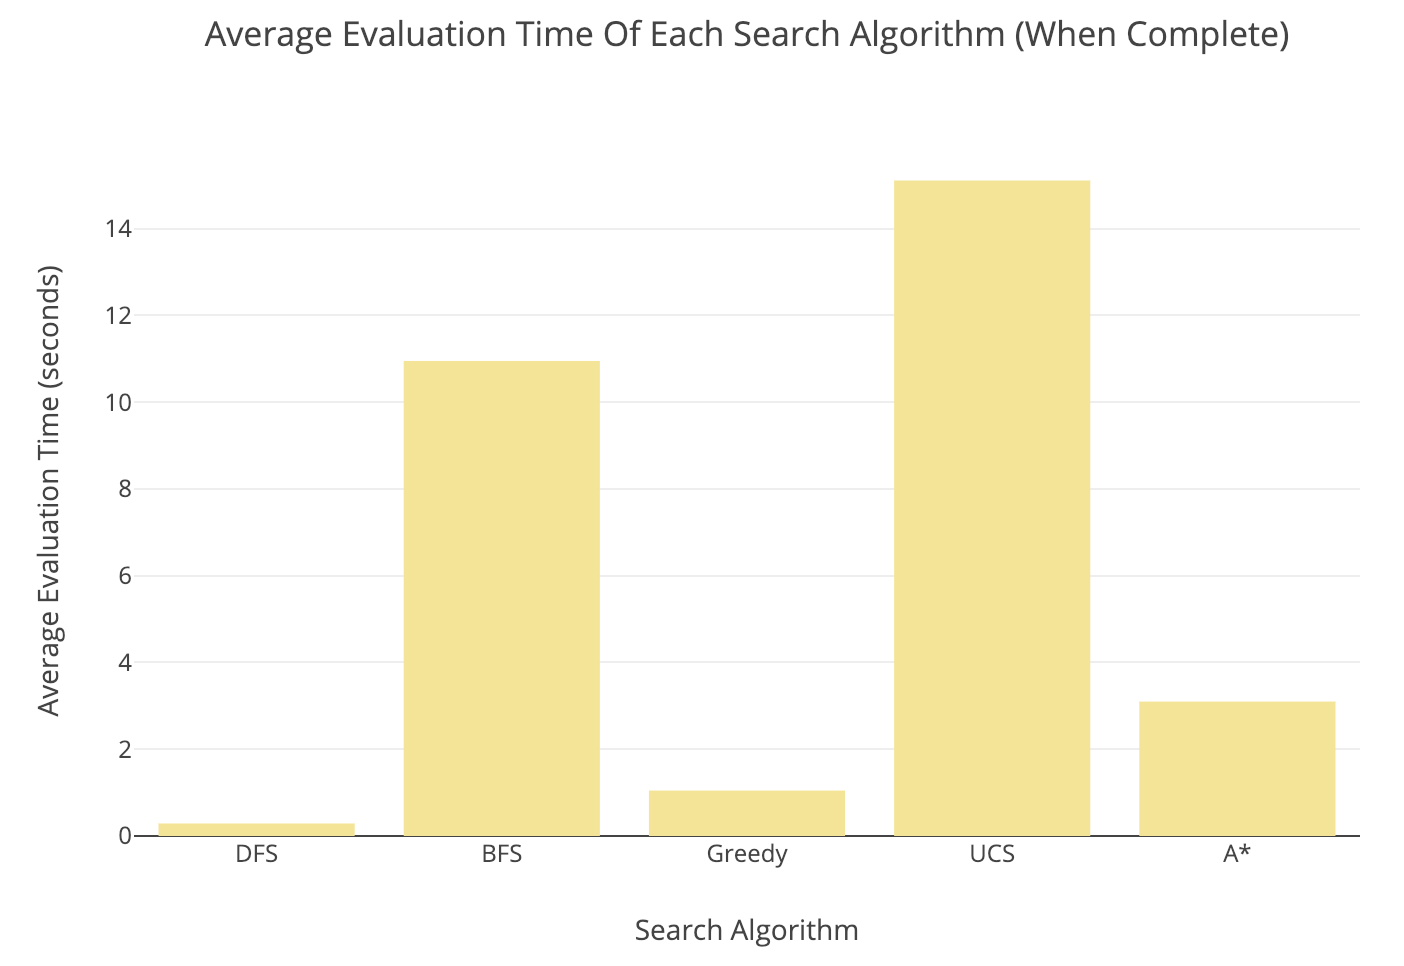
\includegraphics[width=\textwidth]{time_bar.png}
\caption{Average Evaluation Time of Each Search Algorithm}
\end{figure}

\begin{figure}[!h]
\centering
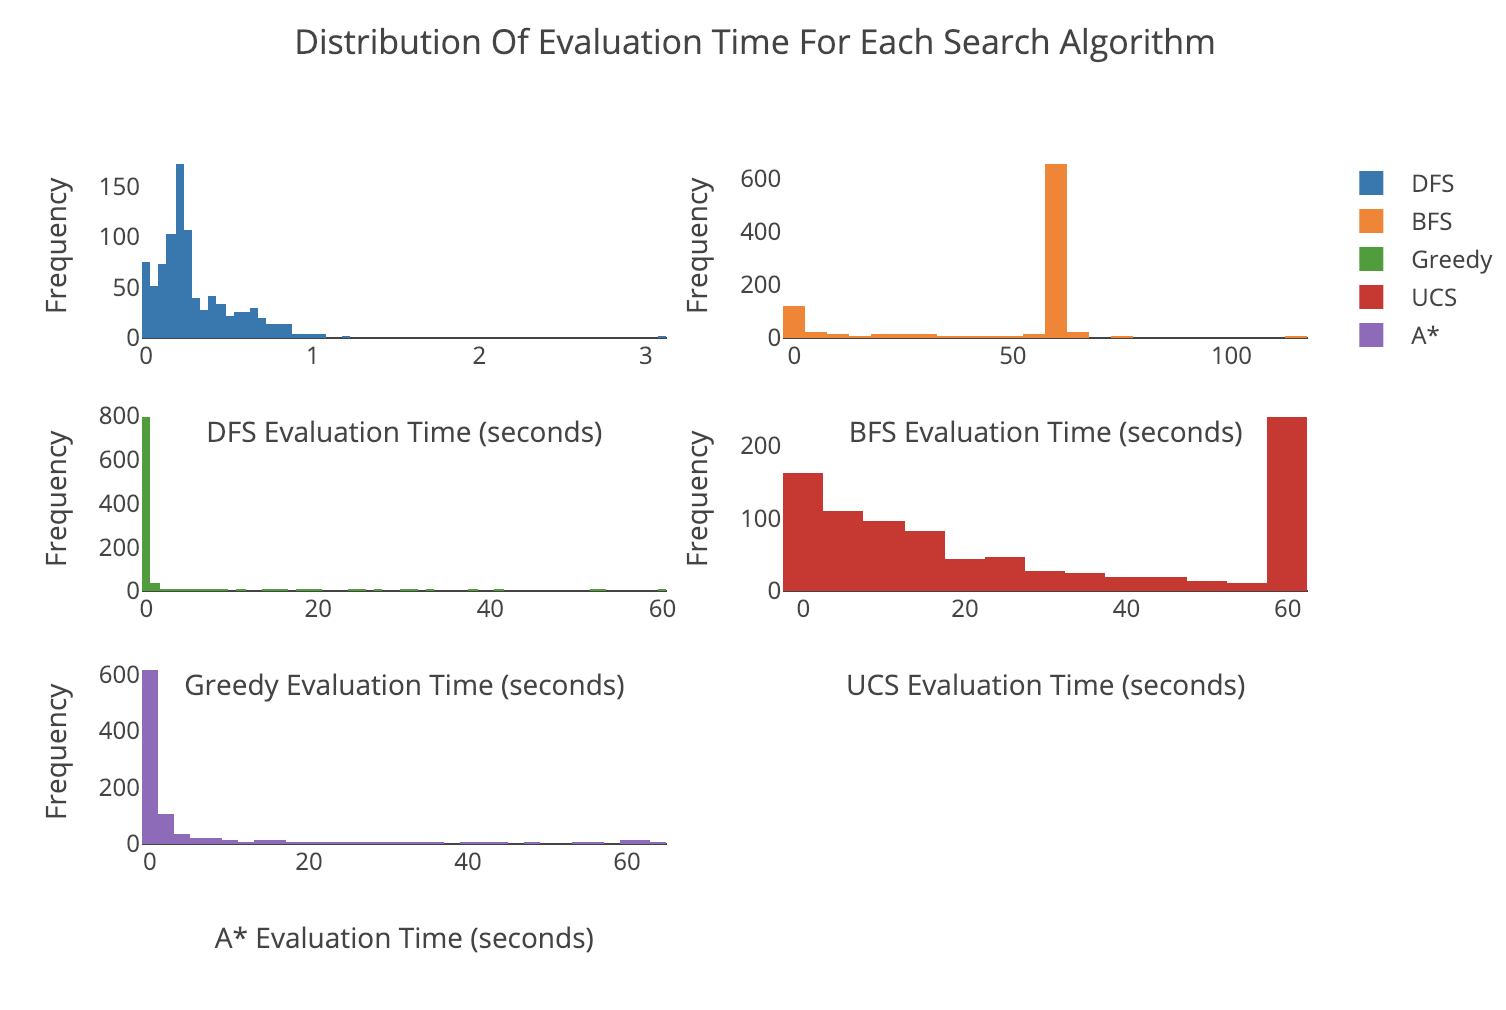
\includegraphics[width=\textwidth]{time_hist.png}
\caption{Distribution of Evaluation Time of Each Search Algorithm}
\end{figure}

\textbf{Sadness}

\textit{Table 3} describes the average sadness that each algorithm incurred on its party when a solution was found. It is important to note that these sadness metrics do not reflect the failure rate described above, and thus, the two should be interpreted together. \textit{Figure 4} shows the graphical representation of this data. To give further context to these point estimates, \textit{Figure 5} shows the distribution of the evaluation time as histograms. Unlike previous tests, these graphs do not show much difference in sadness between algorithms. However, it is again remarkable that \textit{Greedy Search} performed as well as it did: third best, after \textit{UCS} and \textit{A* Search}, both of which were deemed unusable by previous tests of failure rate and evaluation time. The distribution of all of the algorithms points to consistency in the quality of the sadness function.

\begin{table}[!h]
  \centering
  \begin{tabular}{l c}
    \toprule
    Algorithm & Average Sadness) \\
    \midrule
    DFS & 28.189 \\
    BFS & 26.998 \\
    Greedy Search & 22.592 \\
    UCS & 16.332 \\
    A* Search & 19.047 \\
    \bottomrule
  \end{tabular}
  \caption{Average Sadness of Algorithms}
\end{table}

\begin{figure}[!h]
\centering
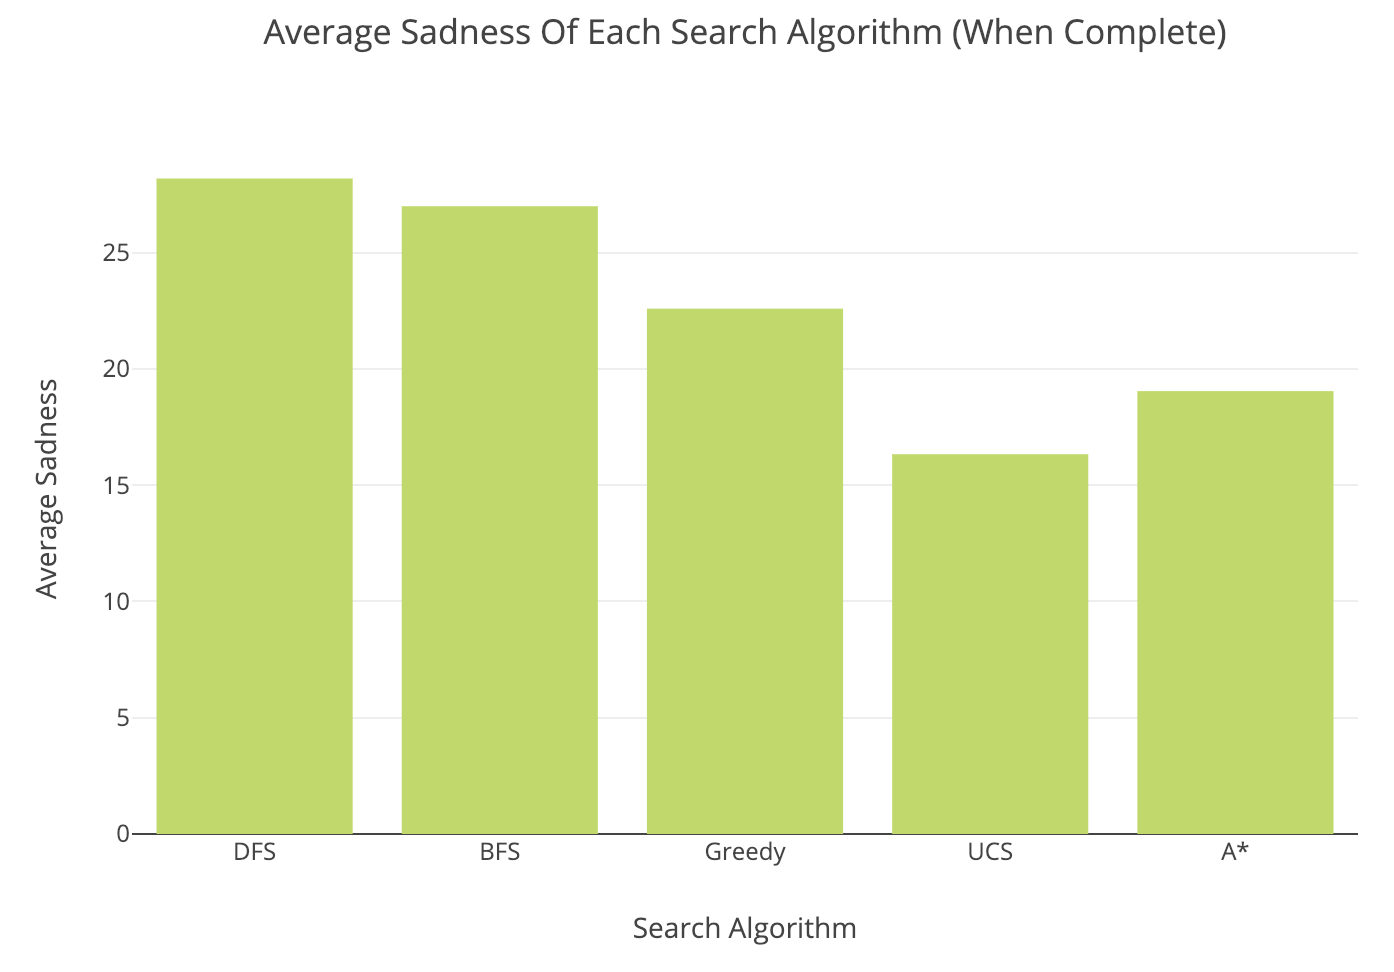
\includegraphics[width=\textwidth]{sad_bar.png}
\caption{Average Sadness of Each Search Algorithm}
\end{figure}

\begin{figure}[!h]
\centering
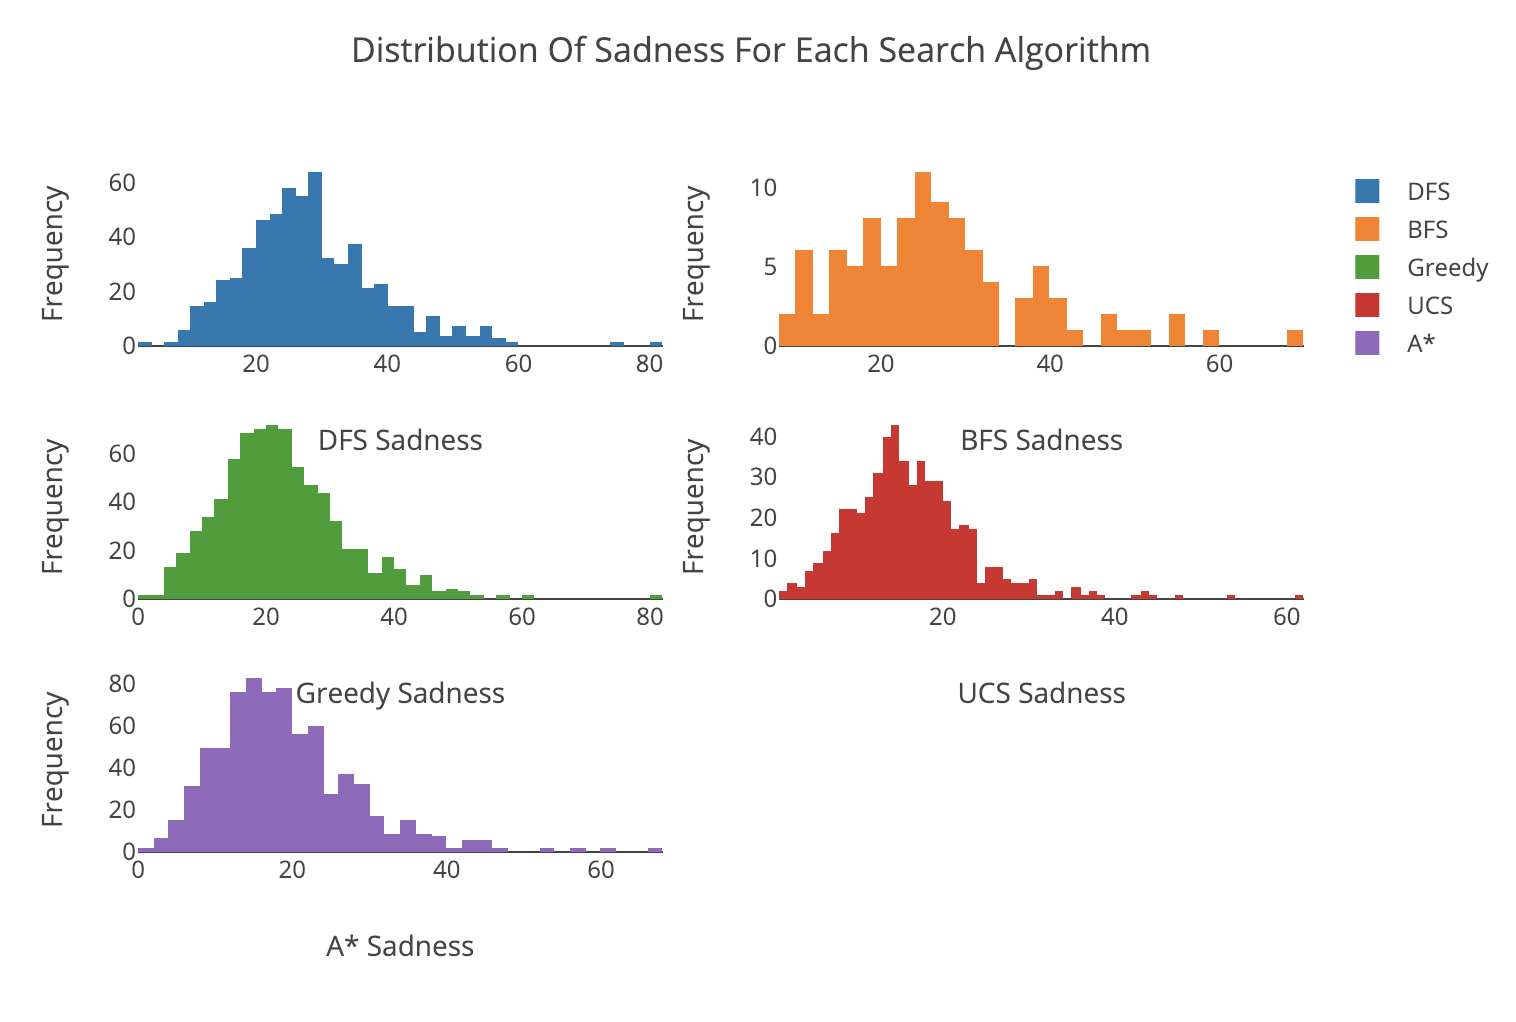
\includegraphics[width=\textwidth]{sad_hist.png}
\caption{Distribution of Sadness of Each Search Algorithm}
\end{figure}

All of the test point to the following conclusion: \textit{Greedy Search} is the best algorithm for \textit{OTT}. Not only is it reliable (proxied by a low failure rate), but it is also fast and effective.


\section{Discussion}

The original intention for this problem was encoding it as a Constraint Satisfaction Problem (CSP). After much investigation, testing, and discussion, the developers decided that the parameters of the problem fit better as a search rather than a constraint satisfaction problem. Instead of morphing constraints into the traditional structure of a CSP, one can use a much more intuitive approach to encode the problem as a search, described in detail in the \textbf{Problem Specification} and \textbf{Approach} sections. Specifically, the problem is structured as a tree search problem, with each node representing a particular venue being added to the list of solutions. Successors are created by the $similarity$ function. To solve the newly specified search problem, the developers considered $5$ algorithms to perform the search: \textit{Depth-First Search (DFS), Breadth-First Search (BFS), Uniform Cost Search (UCS), Greedy Search, and A* Search}. Their performance on this problem is described below.

\textit{DFS} runs quickly and fails infrequently, as it merely has to manoeuvre the tree to find a list of appropriate length, $7$ (the goal test). However, the quality of the solution (proxied by the average $sadness$) is poor compared to the other algorithms because it does not take the cost of a path into account.

\textit{BFS} takes a significant amount of time, and fails very often. Because it expands each level first and the branching factor (the average number of successors generated) is relatively large, \textit{BFS} must traverse a very large number of nodes before reaching depth $7$, the goal. For example, let the initial list of venues be $20$, and let the $similarity$ function filter out $2$ elements from the remaining list at each level. The first level would add $20$ elements to the frontier to be evaluated, each with 18 successors. Each of their successors would have $16$ children, etc. Thus, there would be $(20)+(18*20)+(16*18*20)+(14*16*18*20)+(12*14*16*18*20)+(10*12*14*16*18*20)+1 = 10,731,261$ nodes expanded before reaching the goal. The initial list is typically far more than $20$ nodes, making this problem often unfeasible using \textit{BFS}.

\textit{UCS} runs quickly, but fails relatively frequently (with the second highest rate after \textit{BFS}). It utilizes the $sadnessFunction$ described in the \textbf{Approach} section above as a cost function to generate the priority for each element in its priority queue. Thus, it effectively produces diverse lists of $7$ venues that are located around the users' center point and balance the users' preferences. The weights that were assigned by the developers in the $sadnessFunction$ are fundamental to the algorithm's efficiency and effectiveness. 

\textit{A* Search} and \textit{Greedy Search} both incorporate heuristics to order their frontiers (priority queues). As discussed above in the \textbf{Approach} section, \textiT{A* Search} uses the following linear combination of the heuristic, $h(x)$, and the cost, $c(x)$, to determine the priority of a successor, $x$: $f(x) = h(x) + c(x)$. \textit{Greedy Search} uses the function $c(x)$ to determine the priority of a successor, $x$. 

Finding a consistent (monotonic) heuristic for search problems is a fundamentally difficult problem and a topic of ongoing research.\cite{heuristic}. For this specific problem, that difficulty is augmented by the fact that the goal test is determined by the length of the list instead of the properties of the final node in the path. With that said, a heuristic that performs relatively well was developed and is described in \textbf{Algorithm 2}.

If this heuristic were either consistent or admissible, one would see reliably better performance by the \textit{A* Search} and \textit{Greedy Search} algorithms over \textit{DFS}, \textit{BFS}, and \textit{UCS} algorithms. This seems to be the case, given the results described in the \textbf{Results} section above. Both \textit{A* Search} and \textit{Greedy Search} perform better (they are faster, fail less frequently, and have lower sadness metrics) than the other three algorithms.

\textbf{Greedy Search} consistently out-performed all other algorithms in many metrics, pointing to the conclusion that the heuristic is good, and with \textit{A* Search} near it in performance, the $sadnessFunction$ is a reliable cost function.

Based on the evaluation of the $5$ algorithms on test data relevant to this problem, the developers chose \textit{Greedy Search} as the algorithm for the \href{https://github.com/acamara1498/OTT}{production version of OTT}.

Development of this application will continue, and the following are future development goals:
\begin{itemize}
    \item develop a consistent heuristic for \textit{A* Search} and \textit{Greedy Search}
    \item allow users to specify their own weights for their preferences
    \item tweak the $sadnessFunction$ to include user-defined weights for preferences
    \item allow users to vote on outputted solutions, and incorporate those votes into a long-term model that tweaks $sadnessFunction$ and the $similarity$ function over time
    \item create a mobile application, and allow users to invite each other ahead of time via email and text message
    \item find a more sustainable way of making API calls to the \href{https://developers.google.com/places/web-service/intro}{Google Places API}. The current implementation (under the free tier of Google Cloud Platform) limits these calls
    \item sell this product to Google
\end{itemize}

\newpage

\appendix

\section{System Description}

\textbf{On The Town (OTT)} exists at a public repository on GitHub, \href{https://github.com/acamara1498/OTT}{here}. The \texttt{README.md} file includes all the instructions necessary to run the application and perform the tests that generated the output. Those instructions are replicated below.

The core features of this application rely on the \href{https://developers.google.com/places/web-service/intro}{Google Places AP}I, and search algorithms. The stack is as follows:
\begin{itemize}
    \item Backend: Python, Flask, SQL
    \item Frontend: HTML, JavaScript, CSS, Jinja2
\end{itemize}

\textbf{Installation}

\emph{OTT} runs on \href{https://www.python.org/download/releases/2.7/}{Python 2.7}, and requires the following packages, included in the \texttt{requirements.txt} and \texttt{Pipfile} files:
\begin{itemize}
    \item flask
    \item flask-session
    \item requests
    \item werkzeug
    \item requests-cache
    \item redis
    \item jupyter
\end{itemize}

After cloning this repository onto your computer, there are two ways to install these dependencies:
\begin{enumerate}
    \item \href{https://pipenv.readthedocs.io/}{Pipenv} [recommended]. Install \texttt{Pipenv} with \texttt{brew install Pipenv} if you're using Homebrew on MacOS or Linuxbrew on Linux, or \texttt{sudo dnf install pipenv} if you're using Fedora28. Otherwise, navigate \href{https://pipenv.readthedocs.io/en/latest/install/#installing-pipenv}{here} for more instructions. Next, navigate to the root directory of this repository and run \texttt{pipenv install} to install all dependencies at once and create a virtual environment for the project.
    \item \href{https://pip.pypa.io/en/stable/#}{pip}. Download \texttt{pip} from their website with the following command in a Terminal window: \texttt{curl https://bootstrap.pypa.io/get-pip.py -o get-pip.py}. Next, run \texttt{python get-pip.py}. Finally, navigate to the root directory of this repository and run \texttt{pip install -r requirements.txt} to install all dependencies at once.
\end{enumerate}

If you plan to browse through the frontend, you must initialize the database and server as described below:
\begin{itemize}
    \item Ensure that you have deleted \texttt{users.db} in the \texttt{server/} directory.
    \item Run \texttt{db\_init.py}
    \item Run \texttt{redis-server}
\end{itemize}

To run the web application, run \texttt{python app.py} in a new Terminal window. The implementation of the frontend is currently limited by the fact that running it locally does not allow for the sharing of links, which is crucial to the party system. This is easily solved by migrating this product to its own domain, which is the next step of the development process.

\textbf{Algorithm Testing}

There is a file, \texttt{testing.py} that includes tests of all the \emph{OTT} algorithms. This file allows one to check if the parties and users are being instantiated correctly, to investigate the process of that data structure creation, and test each of the algorithms individually. To run this file, type \texttt{python testing.py} into a Terminal window.

While \texttt{testing.py} tests the basic functionality of the application, a Jupyter notebook file was included to perform robust simulations. \texttt{evaluation.ipynb} performs many simulations of each algorithm on random parties. This file was  used to generate the data used in the \textbf{Results} section. The data generated can also be found in the file \texttt{simulation\_results.csv}. While there is an aspect of randomness to the data generation process (parties of random properties are instantiated), the data analysis process can be replicated by running the \texttt{analysis.ipynb} file, which utilizes the data the developers generated.

As mentioned in the \textbf{Results} and \textbf{Discussion} sections, \textit{BFS} takes a very long time to run, so there were time limits imposed on its evaluation. These time limits are fungible, and one may also opt to not test \textit{BFS} by removing or commenting out the lines of code that respond to its evaluation. For an idea of how long these may take, the developers performed overnight trials to gather the included data.

\newpage

\section{Group Makeup}

\textbf{The Developers}

The following are the three developers of \textbf{On The Town (OTT)} and their major contributions and responsibilities:
\begin{itemize}
    \item Hakeem Angulu, Harvard College 2020, \href{mailto:hangulu@college.harvard.edu}{hangulu@college.harvard.edu}
    \begin{itemize}
        \item Documentation and commenting
        \item UI and UX design and implementation
        \item Algorithms design and implementation
        \item Heuristic design and implementation
        \item Database design and implementation
        \item Backend (Flask and Jinja2) design and implementation
    \end{itemize}
    \item Louie Ayre, Harvard College 2020, \href{mailto:layre@college.harvard.edu}{layre@college.harvard.edu}
    \begin{itemize}
        \item Algorithms design and implementation
        \item Cost function design and implementation
        \item Random party generation for testing and simulations
        \item Diagnostics and empirical value determination
    \end{itemize}
    \item Amadou Camara, Harvard College 2020, \href{mailto:acamara@college.harvard.edu}{acamara@college.harvard.edu}
    \begin{itemize}
        \item Algorithms design and implementation
        \item Testing of the Center.py and the Algorithms
        \item Google Places API Implementation and Usage
        \item Unifying the modules for seamless operation
        \item Documentation and commenting
    \end{itemize}
\end{itemize}

\newpage

\bibliographystyle{plain} 
\bibliography{references}

\end{document}
